\documentclass[12pt]{article}
\usepackage{graphicx}
\pagestyle{empty}

\oddsidemargin  -0.5 cm
\evensidemargin 0.0 cm
\textwidth      6.5in
\headheight     0.0in
\topmargin      -1 cm
\textheight=9.0in

\begin{document}

\mbox{ }

\vfill
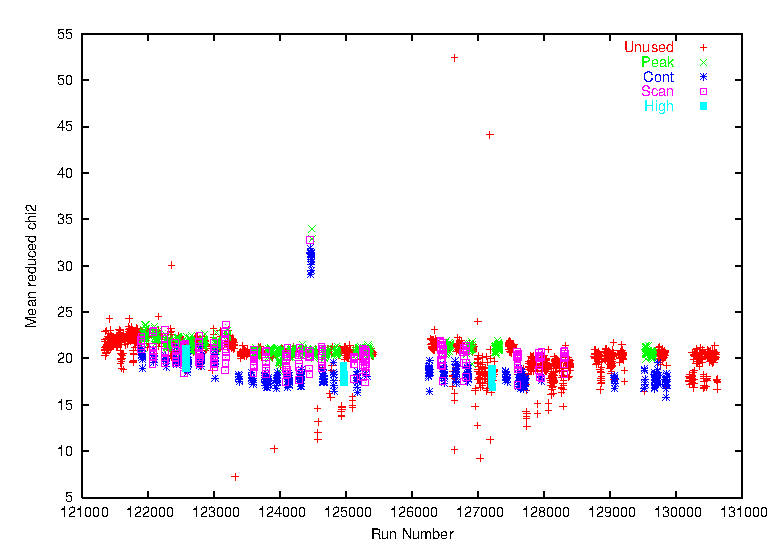
\includegraphics[height=0.9\linewidth, angle=90]{meanredchi.eps}

\vfill
\pagebreak

\mbox{ }

\vfill
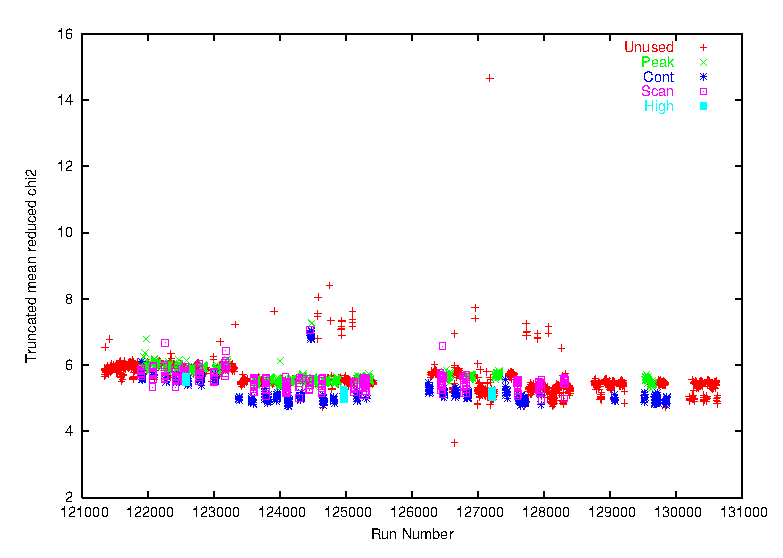
\includegraphics[height=0.9\linewidth, angle=90]{meancutredchi.eps}

\vfill
\pagebreak

\mbox{ }

\vfill
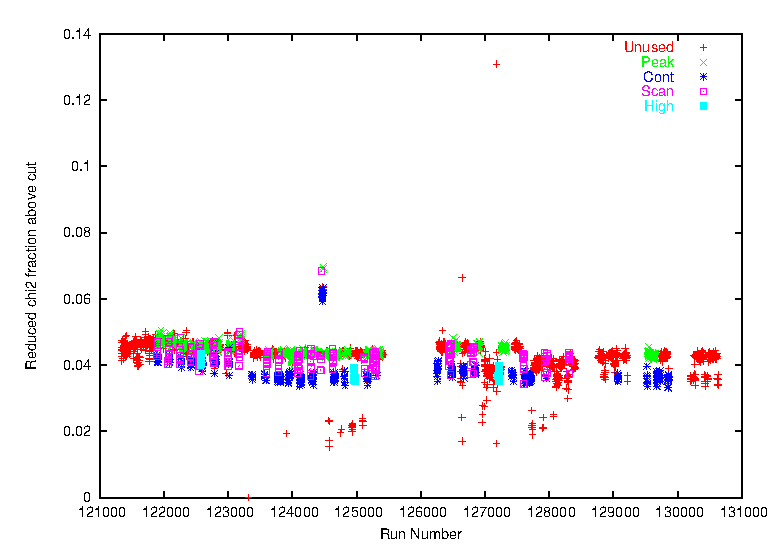
\includegraphics[height=0.9\linewidth, angle=90]{fracredchi.eps}

\vfill
\pagebreak

\mbox{ }

\vfill
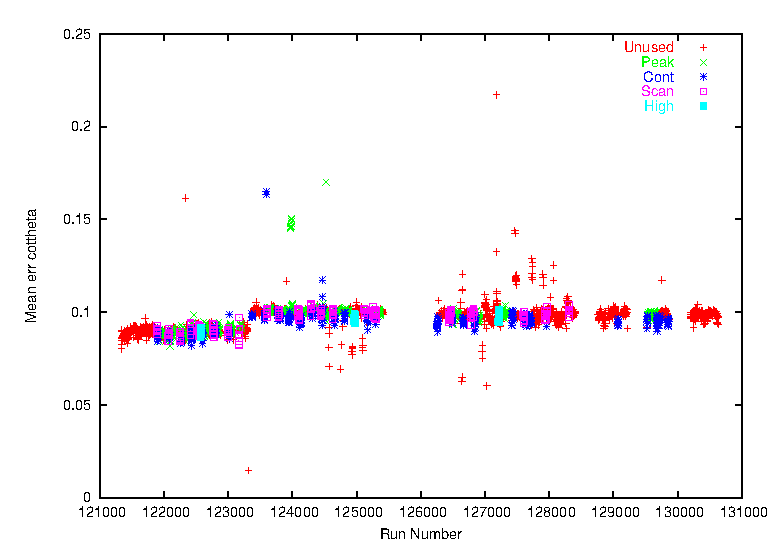
\includegraphics[height=0.9\linewidth, angle=90]{meanerrcotth.eps}

\vfill
\pagebreak

\mbox{ }

\vfill
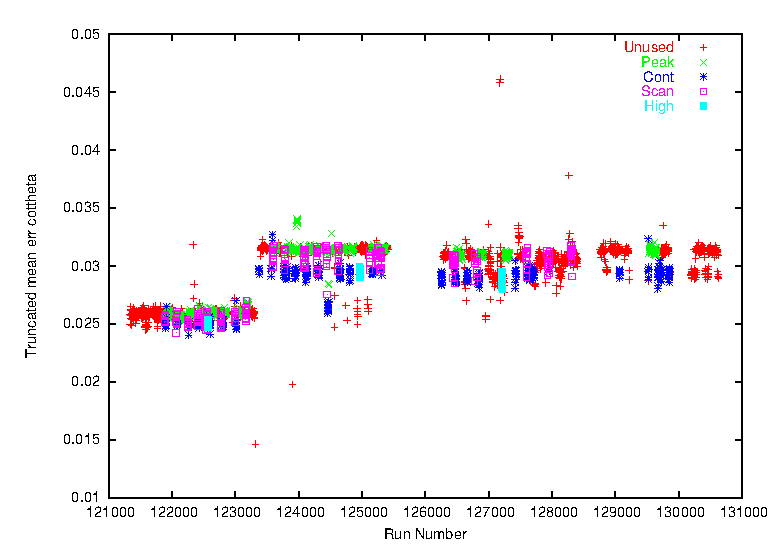
\includegraphics[height=0.9\linewidth, angle=90]{meancuterrcotth.eps}

\vfill
\pagebreak

\mbox{ }

\vfill
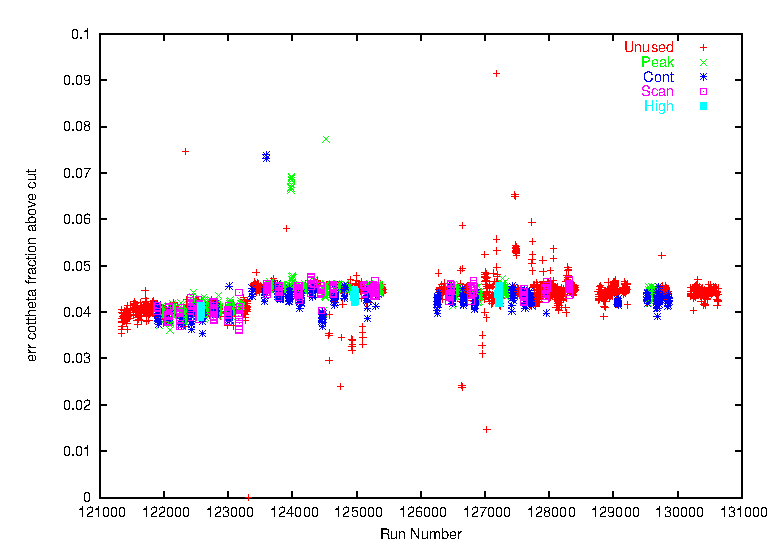
\includegraphics[height=0.9\linewidth, angle=90]{fracerrcotth.eps}

\vfill
\pagebreak

\mbox{ }

\vfill
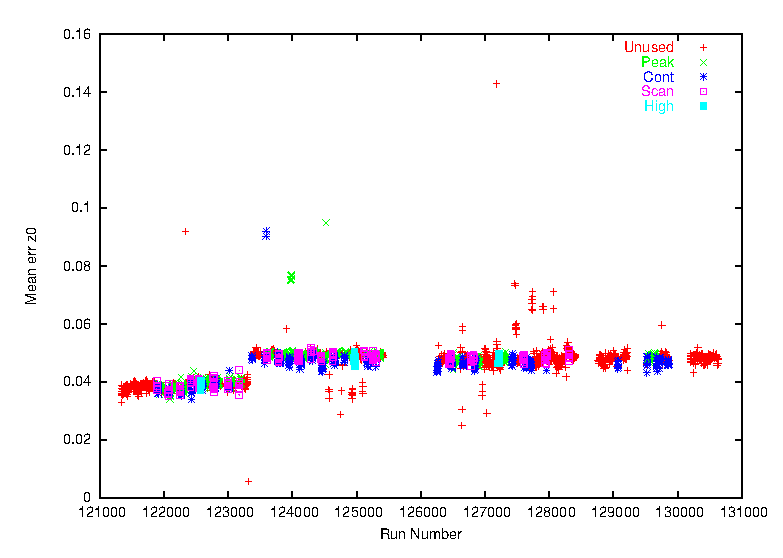
\includegraphics[height=0.9\linewidth, angle=90]{meanerrz0.eps}

\vfill
\pagebreak

\mbox{ }

\vfill
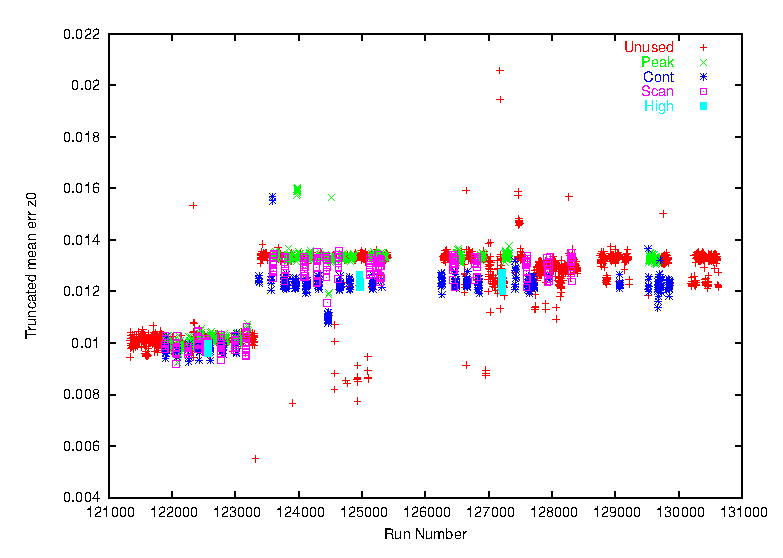
\includegraphics[height=0.9\linewidth, angle=90]{meancuterrz0.eps}

\vfill
\pagebreak

\mbox{ }

\vfill
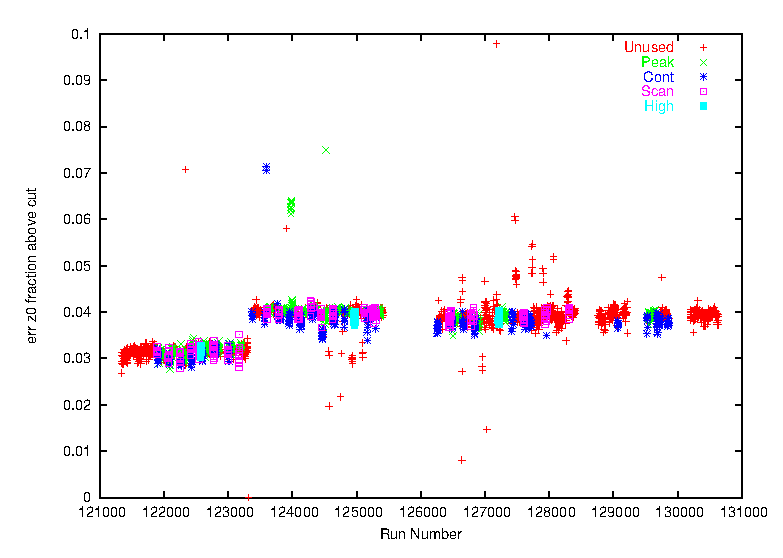
\includegraphics[height=0.9\linewidth, angle=90]{fracerrz0.eps}

\vfill
\pagebreak


\end{document}
